\documentclass{article}

\usepackage[T1]{fontenc}
\usepackage[utf8]{inputenc}
\usepackage[french,english]{babel}

%% This package is necessary to use \includegraphics.
\usepackage{graphicx}

%% This package is necessary to define hyperlinks.
\usepackage{hyperref}

%% These packages are necessary to include code.
\usepackage{listings}
\usepackage{minted} % colored

%% This package is needed to enchance mathematical formulas.
\usepackage{amsmath}



% This is a comment line in latex

% Latex allows you to define your own "commands",
% better known as "macros" in the Latex world.
% The following line is an example of such definition.
\newcommand{\latex}{\LaTeX}


% The next lines contain some meta informations about this document.

\title{Intermediate report for Projet long\\ Due date February 28, 2023}
%\subtitle{A minimal demonstration of \latex}

\author{Giovanni Bernardi, Emmanuel Bigeon, Aldric Degorre}


%% Here we begin giving the actual content o the document.
\begin{document}
\maketitle

\selectlanguage{english}

\section{Introduction}
To obtain a partial grade for \foreignlanguage{french}{``Projet Long''}
you have to write an intermediate report.
The reason to use \latex\ for this is that it greatly simplifies technical writing,
in that it forces authors to work on the {\em content} of the documents,
while \latex\  itself takes care of the {\em appearance} of the documents.

This document shows \latex\  capabilities via a series of minimal
examples (Section~\ref{sec:latex-examples}). Checkout the source file {\tt
  report.tex} to see yourself how it works.
%% We also give you the specs for the
%% intermediate report (Section~\ref{sec:specs-report}) your group has to {\bf
%% submit on February 28, 2023}.

\section{\latex\  examples}
\label{sec:latex-examples}
\latex\  supports automatic hyphenation for many different languages,
and languages can be easily changed even within a single document,
\selectlanguage{french}
par exemple nous voici passés au Français. Le document pourrait continuer ainsi,
mais comme nous avons commencé en Anglais,
\selectlanguage{english}
let us switch back to English.

An empty line in the source file is sufficient for \latex\  to
recognise the beginning of a new paragraph (and this very
paragraph is an example). If you like you can introduce explicitly
a paragraph as follow.

\paragraph{Let's change topic.} In this paragraph we discuss figures
and images. \latex\  manages many different file formats for images.
For example Figure~\ref{fig:geant} shows the network of European universities,
and the image in contained in a {\tt png} file.
The original picture can be found on the \href{https://www.geant.org/}{GEANT web page}
\footnote{In passing, observe that we just gave an example of hyperlink a
\latex document, and also of how to define a footnote.}.
The correct way to insert an image in a document is as it is done in this
paragraph: define a figure environment together with a label, and a caption,
and then use the macro {\tt ref} and the label in the running text
to discuss the image. The horizontal lines above and below the caption in
Figure~\ref{fig:geant} are there just for readability.

\begin{figure}
\label{fig:geant}
\hrulefill
\begin{center}
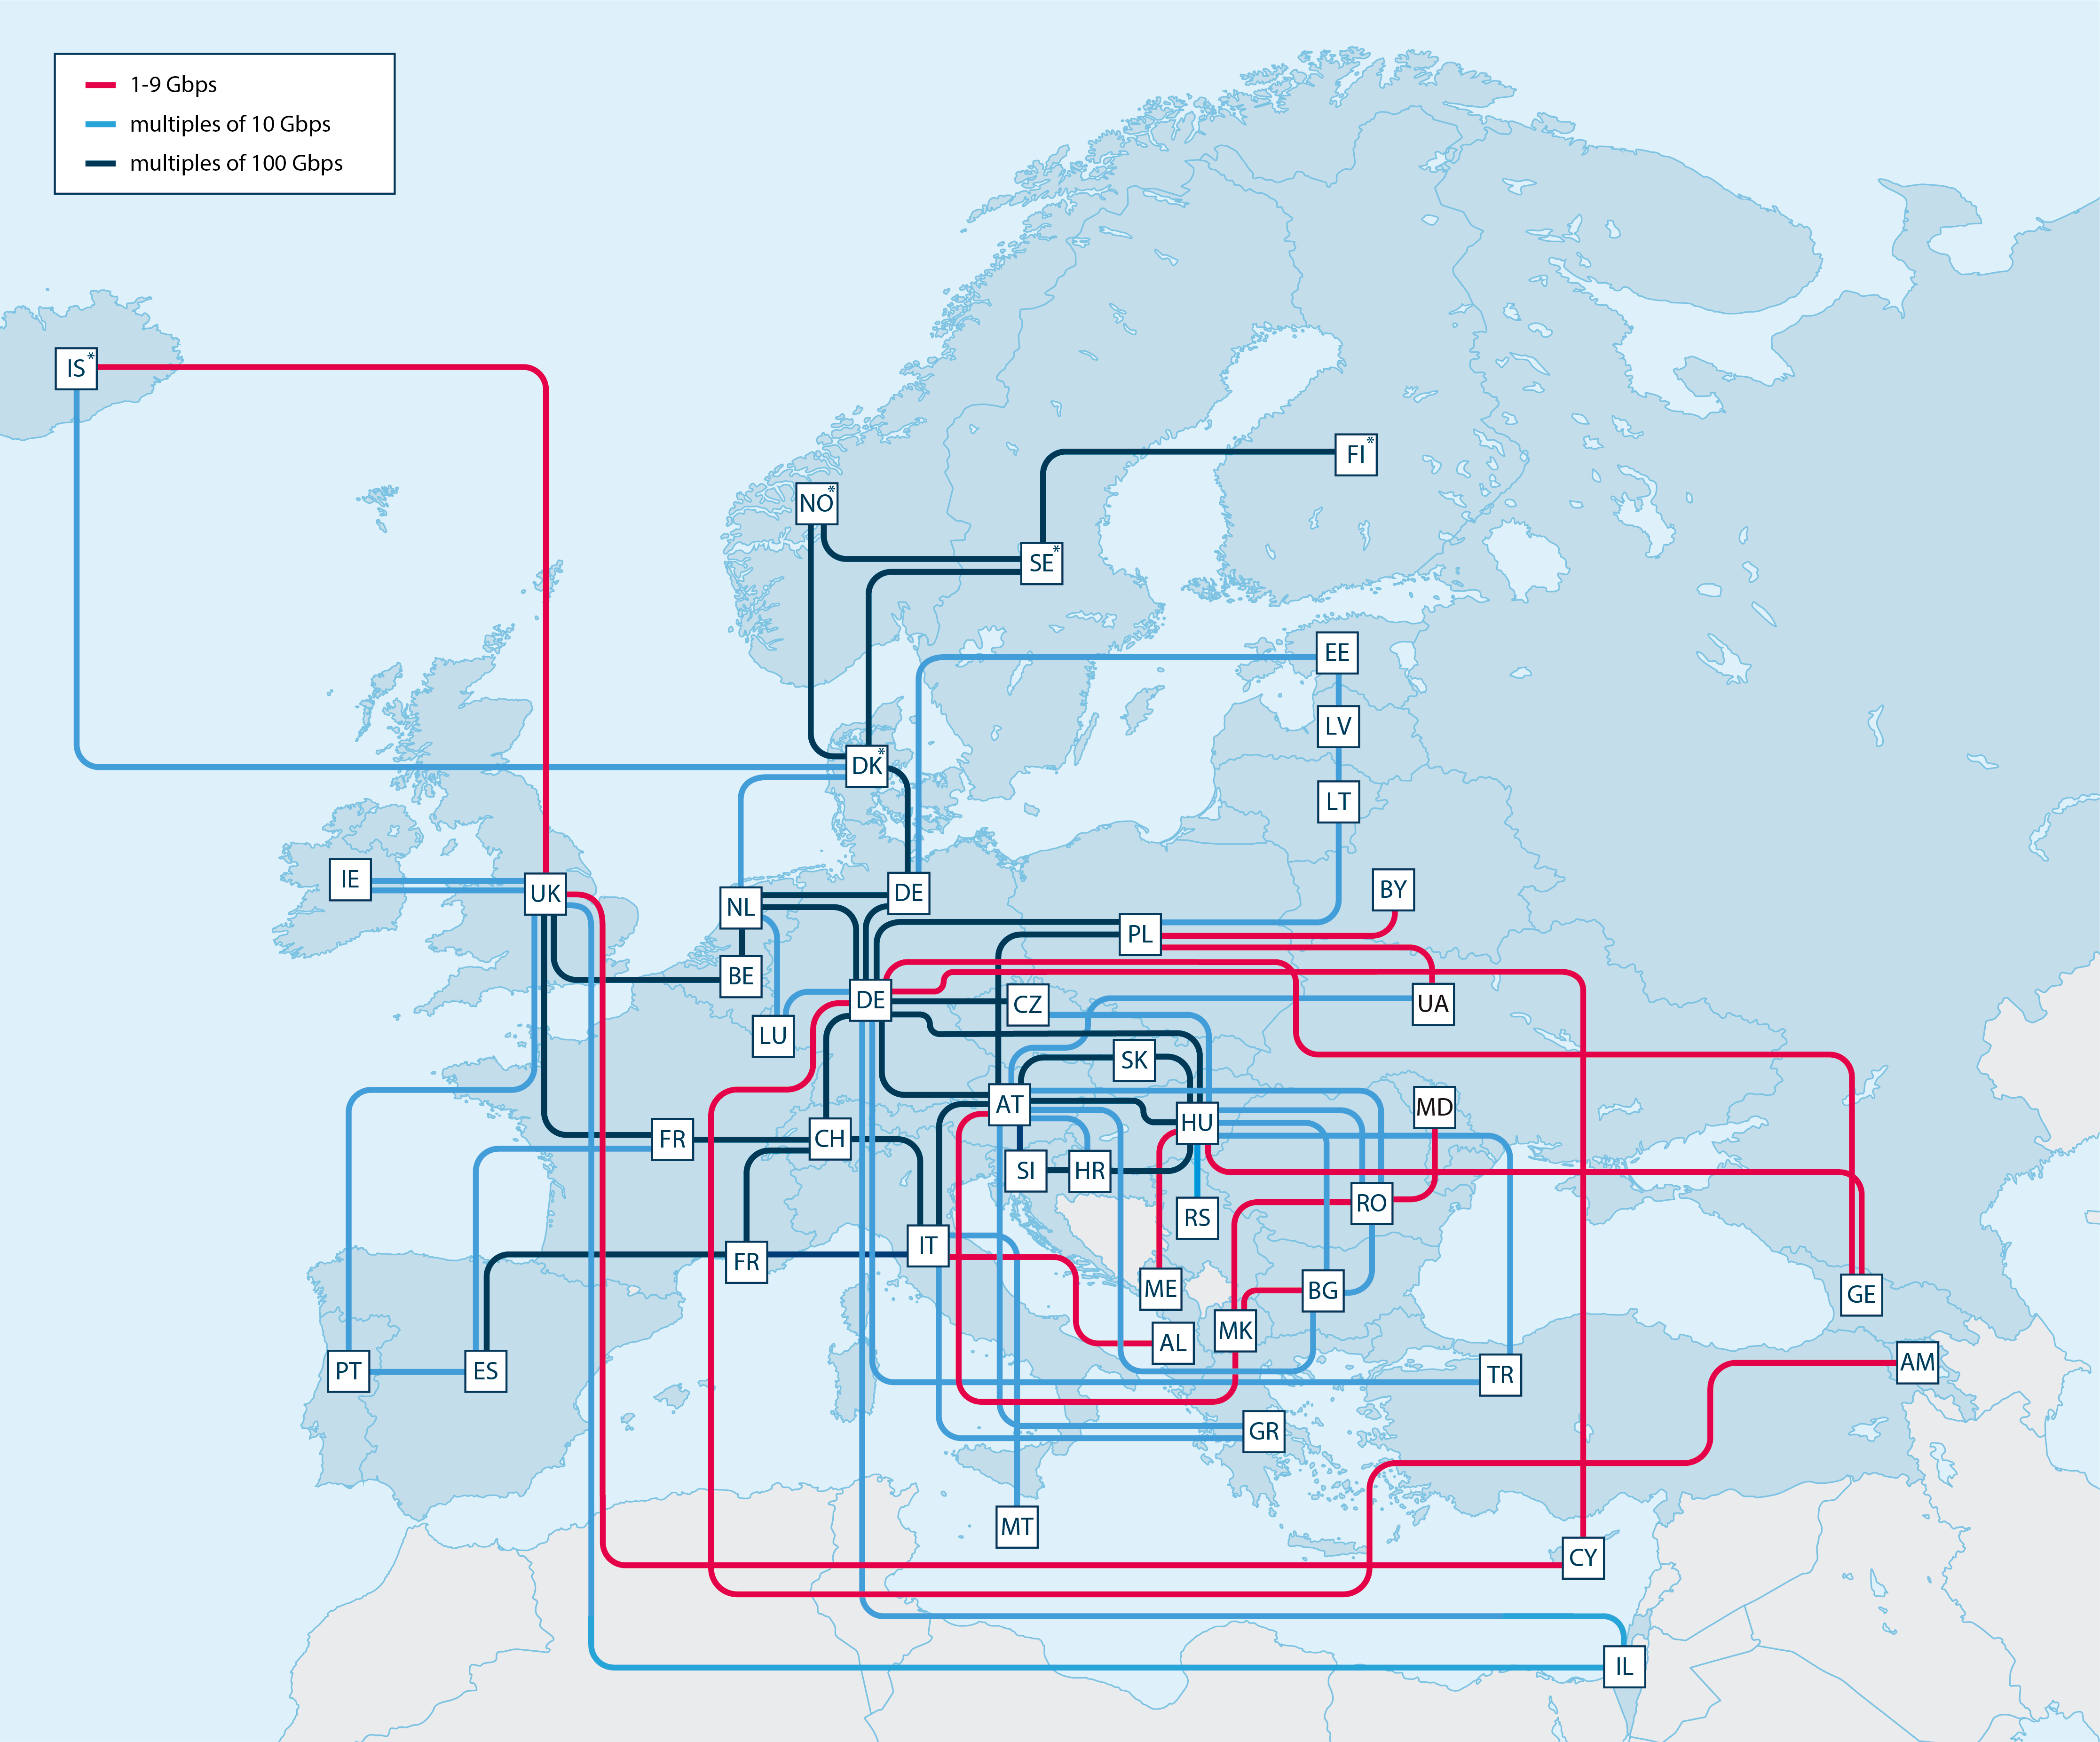
\includegraphics[height=133px,width=200px]{geant}
\end{center}
\caption{A picture of the GEANT network.}
\hrulefill
\end{figure}


Now we change topic again, so we begin a new paragraph.
Indeed, each paragraph in a document should have one clear
topic. Here we showcase a little mathematics. \latex\  has macros to typeset
formulas in the running text, for instance
$ ( (x_1 - x_2)^2 + (y_1 - y_2)^2 )^{\frac{1}{2}}$
is the distance between two points $(x_1,y_1)$ and  $(x_2,y_2)$.
Formulas can also be separated from the running text, in particular
to increase readability. For instance the convective form of the
Navier–Stokes momentum equation is

%% Math formulas separated from the text has to be wrapped between $$ ... $$ or the equation environment
$$
\rho\frac{D{\mathbf u}}{D t} = \rho \left(\frac{\delta {\mathbf u}}{\delta t} + {\mathbf u} \cdot \nabla {\mathbf u} \right) = -\nabla p + \nabla \cdot \left\{ \mu (\nabla \mathbf{u} + (\nabla\mathbf{u})^{T} - \frac{2}{3}(\nabla\cdot\mathbf{u}){\mathbf I} ) + \zeta(\nabla\cdot\mathbf{u}){\mathbf I} \right\} + \rho{\mathbf g}
$$

The formula above does not fit into the margins of the document.
To solve this problem we can use the {\tt aligned} environment within an {\tt equation} environment, and typeset the formula as follows,

%% Math formulas separated from the text has to be wrapped between $$ ... $$ or the equation environment (you can ommit the '*' to number your equations)
\begin{equation*}
  \begin{aligned}
    \rho\frac{D{\mathbf u}}{D t} & =
     \rho \left(\frac{\delta {\mathbf u}}{\delta t} + {\mathbf u} \cdot \nabla {\mathbf u} \right)\\
     & = -\nabla p + \nabla \cdot \left\{ \mu (\nabla \mathbf{u} + (\nabla\mathbf{u})^{T} - \frac{2}{3}(\nabla\cdot\mathbf{u}){\mathbf I} ) + \zeta(\nabla\cdot\mathbf{u}){\mathbf I} \right\} + \rho{\mathbf g}\\
 \end{aligned}
\end{equation*}

\paragraph{What about listing things.} \latex\ also provides useful environments
to create lists. With no need of additional packages one have the {\tt itemize}
environment for unordered lists, whereas the {\tt enumerate} environment allows
you to create an ordered list. A list item within both of these environments has
do be declared with the command \verb+\item+. Needless to say, one can have a
sub-list as a list item. In this case, \latex\ will automatically choose
different bullet points for your nested items. The following example shows you
how to nest properly your sub-lists inside your list.

\begin{enumerate}
  \item First item
  \item Second item
  \begin{itemize}
    \item Nested item a
    \item Nested item b
    \begin{enumerate}
      \item Deeper level of nesting
    \end{enumerate}
  \end{itemize}
  \item Third item
\end{enumerate}

\latex\  let us include very easily code and pseudo-code in our documents.
For example Listing~(\ref{fibo}) shows a {\bfseries wrong} implementation
of the \href{https://en.wikipedia.org/wiki/Fibonacci\_number}{Fibonacci series}.
The code suffers a problem of overflow: for ${\tt n} >= 47$ the value
computed by the function {\tt fibo} as nothing to do with the {\tt n}th fibonacci number.

\begin{figure} \label{fibo}
\hrulefill
  \lstinputlisting[language=python,caption={A naïve implementation of the Fibonacci series.},label=fibo]{fibo.py}%!
  \hrulefill
\end{figure}

However, if you want to add some colors in your code and highlight it, feel free
to use the {\tt minted} environment. But in this case, you have to compile your
document with the {\em option} {\tt -shell-escape}. You can write your code in
the \latex\ document but you can import it from a file as well. The following
example is the same implementation of the Fibonacci series as in
Listing~(\ref{fibo}) using {\tt minted}.

\inputminted{python}{fibo.py}

\end{document}
